On considère ci-dessous la représentation graphique d'une fonction $f$ définie sur $[-2~;~4]$. On a également tracé sa tangente au point $A$ d'abscisse $-1$.
	
	\medskip
	
	\begin{minipage}{0.46\linewidth}
		\begin{enumerate}
			\item Par lecture graphique, donner la valeur de :
			\begin{enumerate}
				\item $f(3)$
				\item $f'(-1)$
			\end{enumerate}
		\end{enumerate}
		
		\begin{enumerate}[start=2]
			\item On admet que la fonction $f$ est définie sur $[-2~;~4]$ par \quad $f(x)=-x^{2}+2x+8$.
			\begin{enumerate}
				\item Calculer $f'(x)$ pour $x$ appartenant à $[-2~;~4]$.
			
				\item Étudier le signe de $f'(x)$ sur $[-2~;~4]$.
			\end{enumerate}
			\item Donner les variations de $f$ sur $[-2~;~4]$.
		\end{enumerate}
		
	\end{minipage}
	\hfill
	\begin{minipage}{0.5\linewidth}
		\centering
		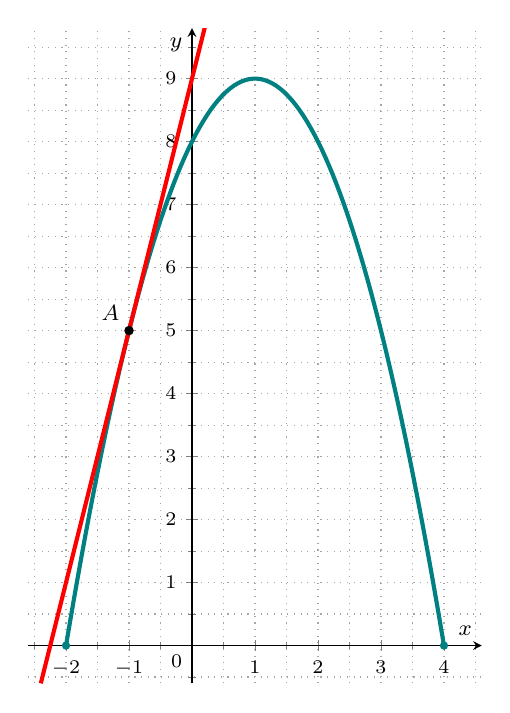
\begin{tikzpicture}
			\begin{axis}[/pgf/number format/.cd, use comma,
				scaled ticks=false,
				x=8mm, y=8mm,
				xmin=-2.6, xmax=4.6, ymin=-0.6, ymax=9.8,
				axis lines=center,
				xtick={-3,-2,-1,0,1,2,3,4,5}, ytick={-1,0,1,2,3,4,5,6,7,8,9,10},
				tick label style={font=\scriptsize},
				minor tick num=1,
				grid=both,
				grid style={gray!70,dotted},
				clip=true]
				\addplot[teal,line width=1.5pt,samples=100,domain=-2:4]{-x^2+2*x+8};
				\fill[teal] (axis cs:-2,0) circle (1.5pt);
				\fill[teal] (axis cs: 4,0) circle (1.5pt);
				\addplot[red,line width=1.5pt,domain=-2.4:0.3]{4*x+9};
				\node[below left,font=\scriptsize] at (axis cs:0,0) {0};
				\node[above left,font=\footnotesize] at (axis cs:-1,5) {$A$};
				\node[font=\footnotesize,above left] at (axis cs:4.6,0) {$x$};
				\node[font=\footnotesize,below left] at (axis cs:0,9.8) {$y$};
				\filldraw (axis cs:-1,5) circle (1.5pt);
			\end{axis}
		\end{tikzpicture}
	\end{minipage}
	
	\medskip
